\documentclass{article}
\usepackage[utf8]{inputenc}
\usepackage{hyperref}

\providecommand{\tightlist}{%
  \setlength{\itemsep}{0pt}\setlength{\parskip}{0pt}}

\title{Carberry Pi Documentation}
\author{Ryan McHugh}
\date{April 2020}

\begin{document}

\maketitle


\begin{center}
\line(1,0){300}
\end{center}


\setcounter{secnumdepth}{2}

% // Logo

\textbf{Carberry Pi}

\begin{verbatim}

         11111111
        11   11   1
     111     11    1111
    111111111111111111111111
    1111001111111111110011111
      100001        100001
        00              00            
\end{verbatim}

\hypertarget{outline-of-this-document}{%
\subsection{Outline of this Document}\label{outline-of-this-document}}

\begin{enumerate}
\def\labelenumi{\arabic{enumi}.}
\item
  \protect\hyperlink{introduction}{Introduction}
\item
  \protect\hyperlink{hardware}{Hardware}
\item
  \protect\hyperlink{software}{Carberry Pi Software}

  3.1 \protect\hyperlink{dashboard}{Dashboard}

  3.2 \protect\hyperlink{diagnostics}{Diagnostics}

  3.3 \protect\hyperlink{configuration}{Configuration}

  3.4 \protect\hyperlink{architecture}{Architecture}
  
\item
  \protect\hyperlink{connecting-the-pieces}{Connecting the Pieces}
\item
  \protect\hyperlink{getting-up-and-running}{Getting Up and Running}
\end{enumerate}

\hypertarget{introduction}{%
\section{Introduction}\label{introduction}}

\begin{itemize}
\tightlist
\item
  \emph{Carberry Pi} is an automotive application of a mini-computer in
  the car. As the quintessential project for my undergraduate studies,
  this concept provides a deep-dive into an area of future interest.
\end{itemize}

\hypertarget{hardware}{%
\section{Hardware}\label{hardware}}

Carberry Pi requires a few tools of the trade.

~~~~Namely:

\begin{itemize}
\item
  Raspberry Pi (this project uses a Raspberry Pi 3 model B)
\item
  Professional Grade OBDII Cable
\item
  Raspberry Pi Touchscreen
\item
 \href{https://thepihut.com/products/mini-rtc-module-for-raspberry-pi}{DS3231 RTC IC}
  (Real Time Clock)
\end{itemize}

\hypertarget{carberry-pi-software}{%
\section{Carberry Pi Software}\label{carberry-pi-software}}

\hypertarget{dashboard}{%
\subsubsection{Dashboard}\label{dashboard}}

\begin{figure}
\centering
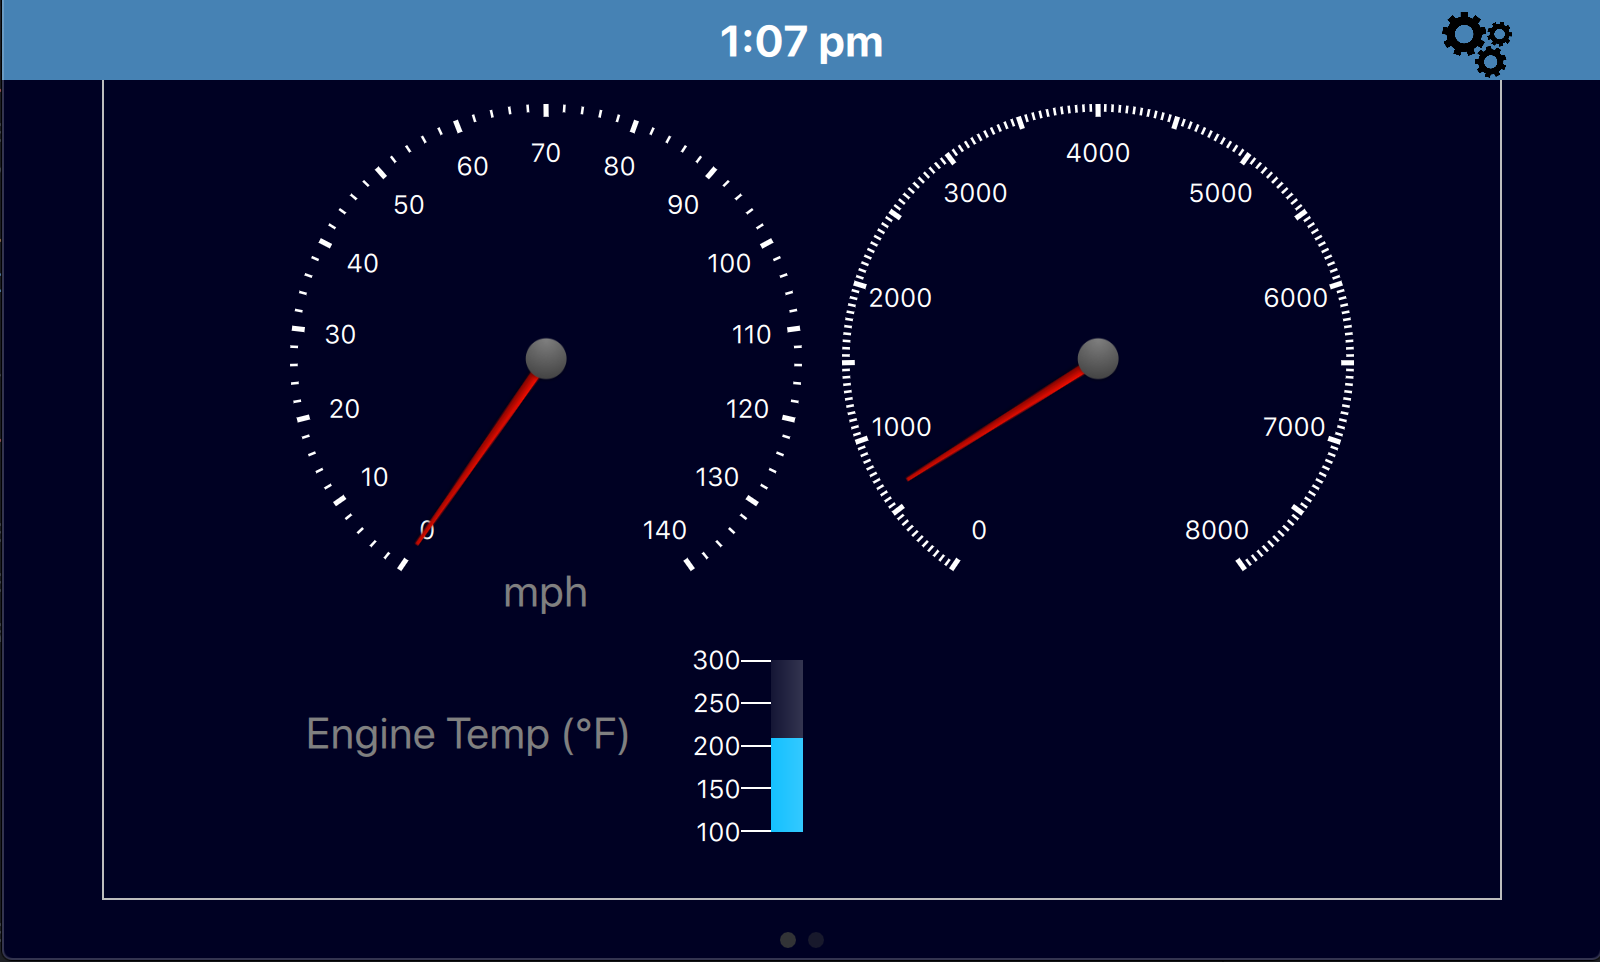
\includegraphics{./resources/dash.png}
\caption{Dashboard}
\end{figure}

\hypertarget{diagnostics}{%
\subsubsection{Diagnostics}\label{diagnostics}}

\begin{figure}
\centering
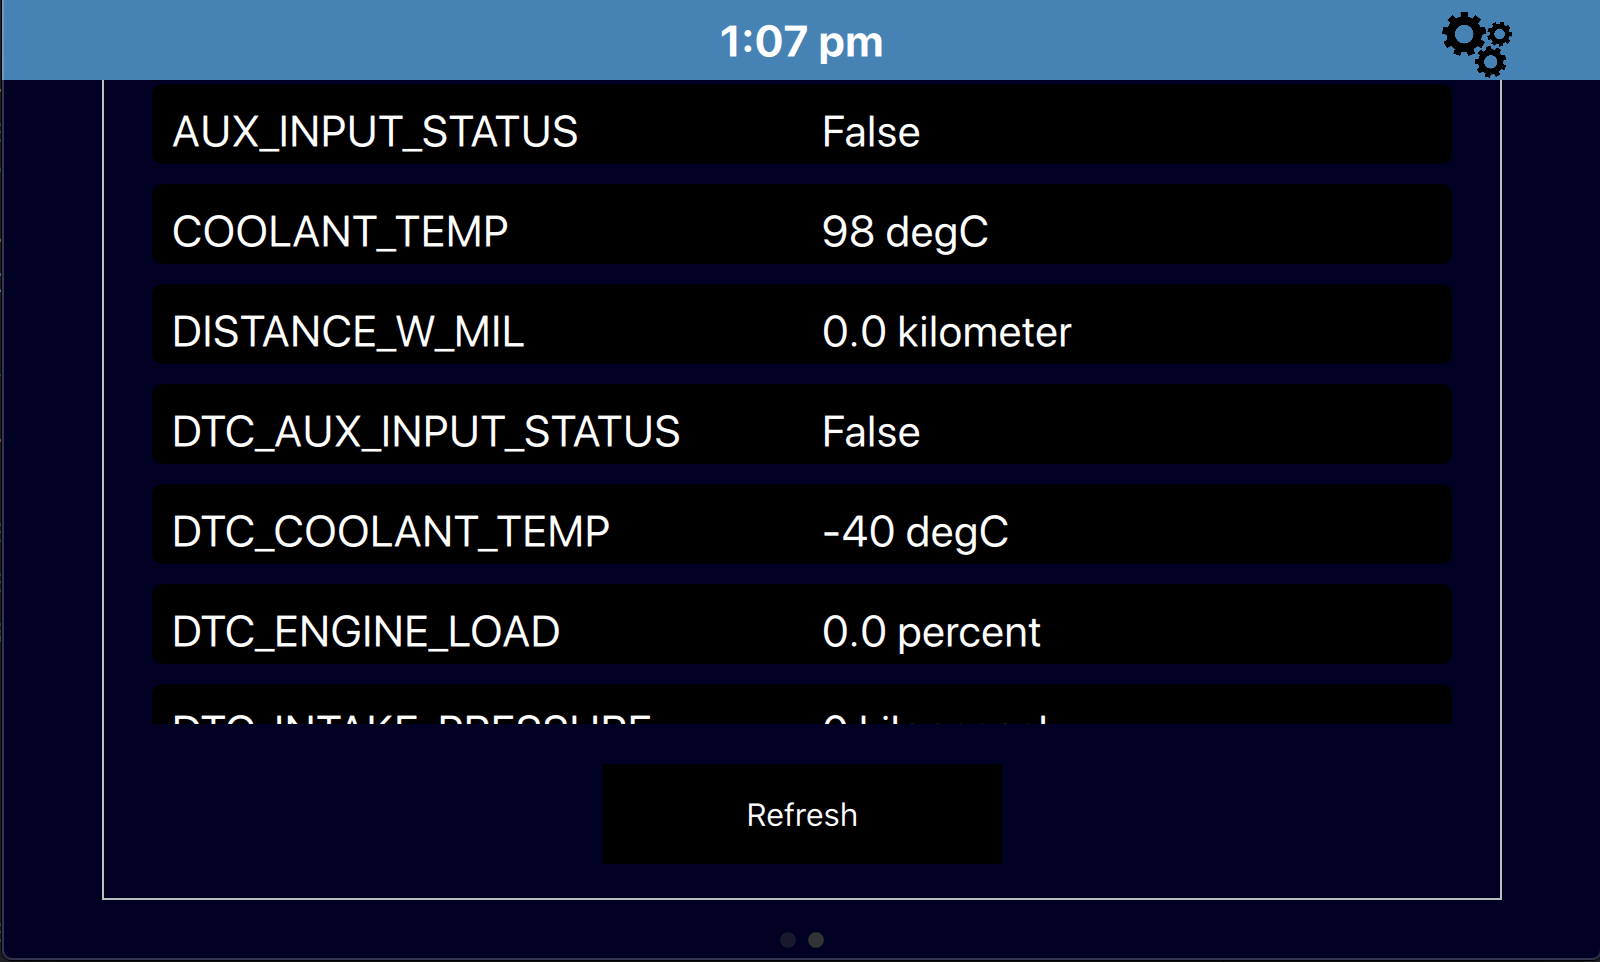
\includegraphics{./resources/diagnostics.png}
\caption{Diagnostics}
\end{figure}

\hypertarget{configuration}{%
\subsubsection{Configuration}\label{configuration}}

\begin{figure}
\centering
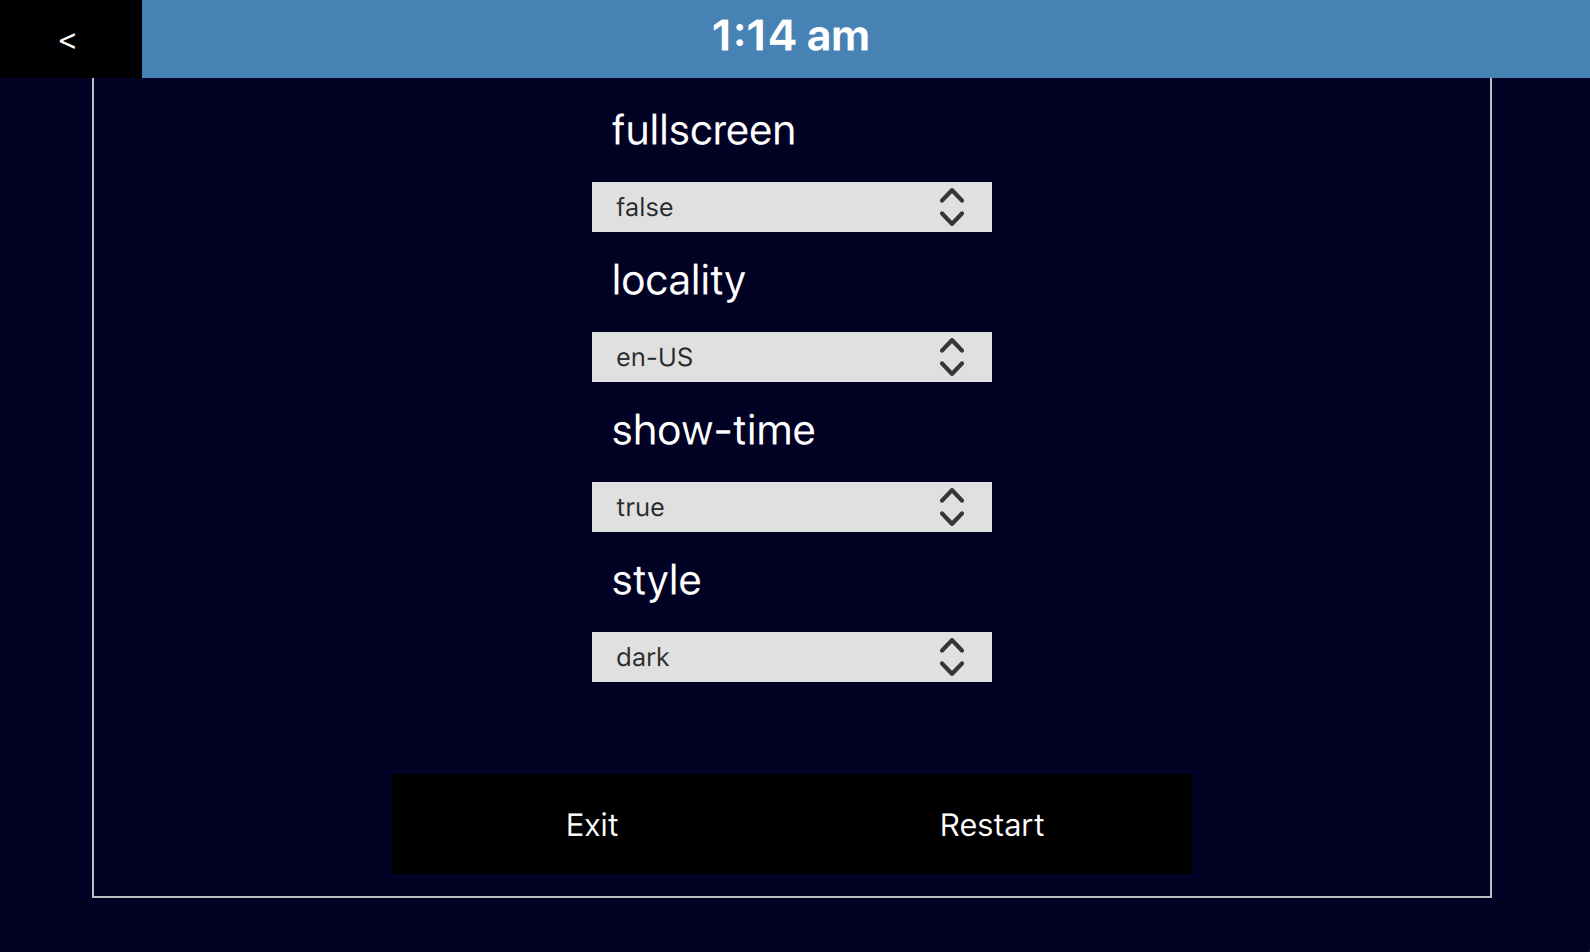
\includegraphics{./resources/configuration.png}
\caption{Configuration}
\end{figure}




\subparagraph{Manage the settings of the application.}

\begin{itemize}
  \item 
    locality: Region-based conversion of units (main dashboard only)
\end{itemize}
\begin{itemize}
  \item 
    fullscreen: Toggle for fullscreen on startup (only works on
\end{itemize}
\begin{itemize}
  \item 
    style: Manages the overall theme of the application (toggle between light and dark modes)
\end{itemize}
\begin{itemize}
  \item 
    time: Show/Hide the time in the header bar
\end{itemize}

\hypertarget{architecture}{%
\subsubsection{Architecture}\label{architecture}}

\hypertarget{toolkit}{%
\subparagraph{Toolkit}\label{Toolkit}}

\begin{itemize}
\item
  Backend: Python

  \begin{itemize}
  \tightlist
  \item
    Utilizes \href{https://python-obd.readthedocs.io/en/latest/}{python-obd} library for OBD information
  \end{itemize}
\item
  Frontend: PyQt (Qt-Quick) + QML \textbar{} Javascript
\end{itemize}

\hypertarget{interface-architecture}{%
\subparagraph{Interface Architecture}\label{interface-architecture}}

\begin{itemize}
\item
  Dynamic loading allows react.js style module instantiation and destruction

  \begin{itemize}
  \item
    Each component is loaded into a \emph{view} as a separate entity
  \item
    These components can then be pushed/popped onto or from the
    main\emph{stackview}
  \item
    A separate script (javascript) manages the creation/destruction of
    the \emph{back} button
  \end{itemize}
\item
  Time

  \begin{itemize}
  \item
    The time is based on the RTC (Real Time Clock) of the Raspberry Pi
    itself.
  \item
    As such, changing the locality has no effect on the time value.
  \end{itemize}
\end{itemize}

\subparagraph{Directory Structure \textbar{} File Enumeration}
\begin{itemize}
    \item \emph{documentation}: Stores the source files and compiled containers for this documentation\\
    \item \emph{src}: Contains the Project Source files

    \begin{itemize}
        \item \emph{items}: reusable \_custom\_ QML items
        \item \emph{js}: JavaScript scripts (primarily for object creation and destruction)
        \item \emph{log}: storage for log output \emph{(YYYY-MM-DD)}
        \item \emph{partials}: QML partials (snippets)
        \item \emph{resources}: assets \textbar{} icons
    \end{itemize}
\end{itemize}



\hypertarget{connecting-the-pieces}{%
\section{Connecting the Pieces}\label{connecting-the-pieces}}

// tutorial with picture layout of connecting each component

\hypertarget{getting-up-and-running}{%
\section{Getting Up and Running}\label{getting-up-and-running}}

\hypertarget{recommended-os-dietpi}{%
\paragraph{Recommended OS: DietPi}\label{recommended-os-dietpi}}

The \href{https://dietpi.com}{\emph{DietPi}} (debian-based) operating system distribution acts as a
lightweight desktop environment for running GUIs on the Pi.

\begin{flushleft}
Of Course, you may run this application on another operating system of
your choosing.
\end{flushleft}



\hypertarget{recommended-de-lxde}{%
\paragraph{Recommended DE: LXDE}\label{recommended-de-lxde}}
This project uses \href{https://wiki.lxde.org/en/Main_Page}{\emph{LXDE}}. It is a lightweight desktop environment
that suits the limited hardware of the Raspberry Pi wonderfully.


\paragraph{The use of another desktop environment will require appending a
command that executes the \emph{start\_carberry.sh} script to the
startup file of the respective DE.}

\subsubsection{Installation}
\begin{enumerate}
    \def\labelenumi{\arabic{enumi}.}
    \item   Clone the repo from \url{https://github.com/brohemz/carberry-pi}
    \item   Run \emph{install.sh} in the \emph{src} folder as SuperUser
    \begin{itemize}
        \item Note: The \emph{autostart} functionality of the installation script
                    requires LXDE.
    \end{itemize}
    \item In order to ensure proper \emph{autostart} functionality, restart the computer now.
    \item Run the application \emph{start\_carberry.sh} from \emph{src} folder.
\end{enumerate}
\paragraph{You should now see the main dashboard.}



\end{document}
